\section{Variability of GRMHD models}\label{app:variability}

%%%%%%%%%%%%%%%%%%%%%%%%%%%%%%%%%%%%%%%%%%%%%%%%%%
%% notes from people who drafted the section

% \bp{Seems like (1) and (2) here are (or will be) discussed more thoroughly in the Numerical Methods appendix.  Given both seem to conclude that all models are consistent, and thus that changing these parameters would not reduce variability, maybe we can refer there instead of re-writing?}
%\monika{11Dec:addressed below}
%==============================================================================
% 1. GRMHD resolution.

% discussion of varying resolution [Ben to spelunk to find a 448 down set of images]

% Discussion of high resolution HAMR model.

% mapping between 230 GHz variability and accretion rate variability
%\monika{11Dec:addressed in B1}

%==============================================================================
%2. Image resolution.
%\monika{11Dec:addressed in B1}
%==============================================================================
%3. Model duration is not sufficiently long.
%KORAL model analysis.
% MM 11 Dec: now in C1
%==============================================================================
%4. $\sigma_{cut}$ is overproducing variability.
% MM 11 Dec: when sigma_cut>sigma_crit  physics is unreliable and this is mentioned in the model section now. maybe not appropriate to discuss here
%==============================================================================
%5. Initial conditions are not a good model.
%Comparison of Monika model initial conditions
% there was nothing added on this to the draft yet
%==============================================================================
% 6. Cooling filters the light curve. [Ben]
% \monika{11Dec:moved at the end: merged into subsection C.2}
%==============================================================================
%7. Electron distribution function model is inadequate.

%a.  Discussion of models with varying electron heating models.  Discussion of Jason's eheating models.   Forward reference to Diaz et al.  [Vedant]

%b. Discussion of models with $\Rl = 10$. [Vedant]
% \monika{11Dec: now in C2}

%%%%%%%%%%%%%%%%%%%%%%%%%%%%%%%%%%%%%%%%%%%%%%%%%%

Nearly all models fail to recover the variability of \sgra in 230\GHz flux density as measured by \mi{3}.
In this Appendix we discuss and dismiss four possible causes for this variability excess.

%==============================================================================
\subsection{Simulations Duration}\label{app:narayan}

\begin{figure}
  \centering
  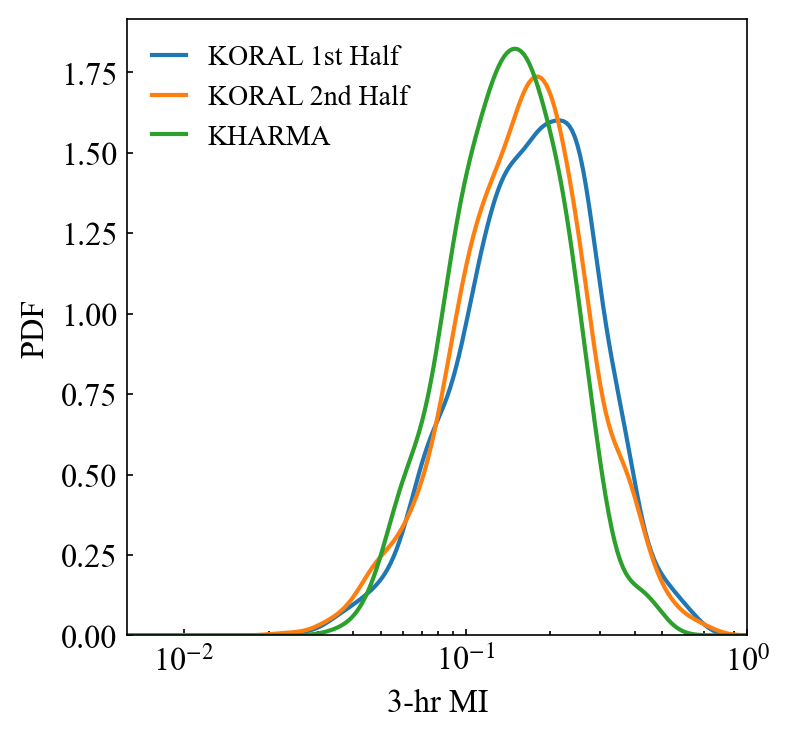
\includegraphics[width=\columnwidth]{./figures/Koral_vs_IL_MI.png}
  \caption{Distribution of \mi{3} from \koral models, divided between the first and second half of the simulation, and from the fiducial \kharma models. We choose the models that are at similar points in the parameter space, limiting the comparison to spin -0.9, -0.5, 0.0 and 0.9 over all inclinations for the \koral models and MAD, \Rh 40, spin -0.94, -0.5, 0.0, and 0.94 for the \kharma models.} 
  %Specifically: \koral models are all MAD, inclination 10, 30, 50, 70, 90, spin -0.9, -0.5, 0.0, 0.9, rhigh 20. \kharma models are MAD, inclination 10, 30, 50, 70, 90, spin -0.94, -0.5, 0.0, 0.94, rhigh 40.
  \label{fig:koral_MI}
\end{figure}

The fiducial models are evolved for $\sim \no{30000}\,\tg$.
Figure ~\ref{fig:koral_MI} compares $\mi{3}$ distributions from a fiducial \kharma simulation to a \koral model with similar parameters that was evolved and imaged for approximately three times longer.
The $\mi{3}$ distributions have similar mean and standard deviation regardless of time interval chosen for comparison.
%The two models displayed in the figure differ in resolution of the numerical grid and initial torus size, consistent with the claim that the variability excess is not driven by numerical resolution or initial conditions of the GRMHD simulations.

%==============================================================================
\subsection{Effect of \texorpdfstring{$\Rl$}{Rlow}}

The $\Rh$ prescription (Equation \ref{eq:rhigh_prescription}) has three free parameters: $\Rh$, $\Rl$ and $\beta_\mathrm{crit}$.
In the main text the $\Rh$ parameter is varied while $\Rl$ and $\beta_\mathrm{crit}$ are set to unity.

The $\Rl$ parameter determines the electron temperature in regions of low $\beta$, i.e. in and near the funnel.
Increasing $\Rl$ mimics rapid electron cooling.
We are particularly interested in the effect of increasing $\Rl$ on \mi{3}.

Figure~\ref{fig:mi_rlow} shows the \mi{3} distribution for a set of four \kharma models with four values of $\Rl$ (1,2,5, and 10).
Evidently the \mi{3} distribution does not exhibit a clear trend with $\Rh$, and is still inconsistent with the observed distribution even at $\Rl = 10$.

\begin{figure*}
  \centering
  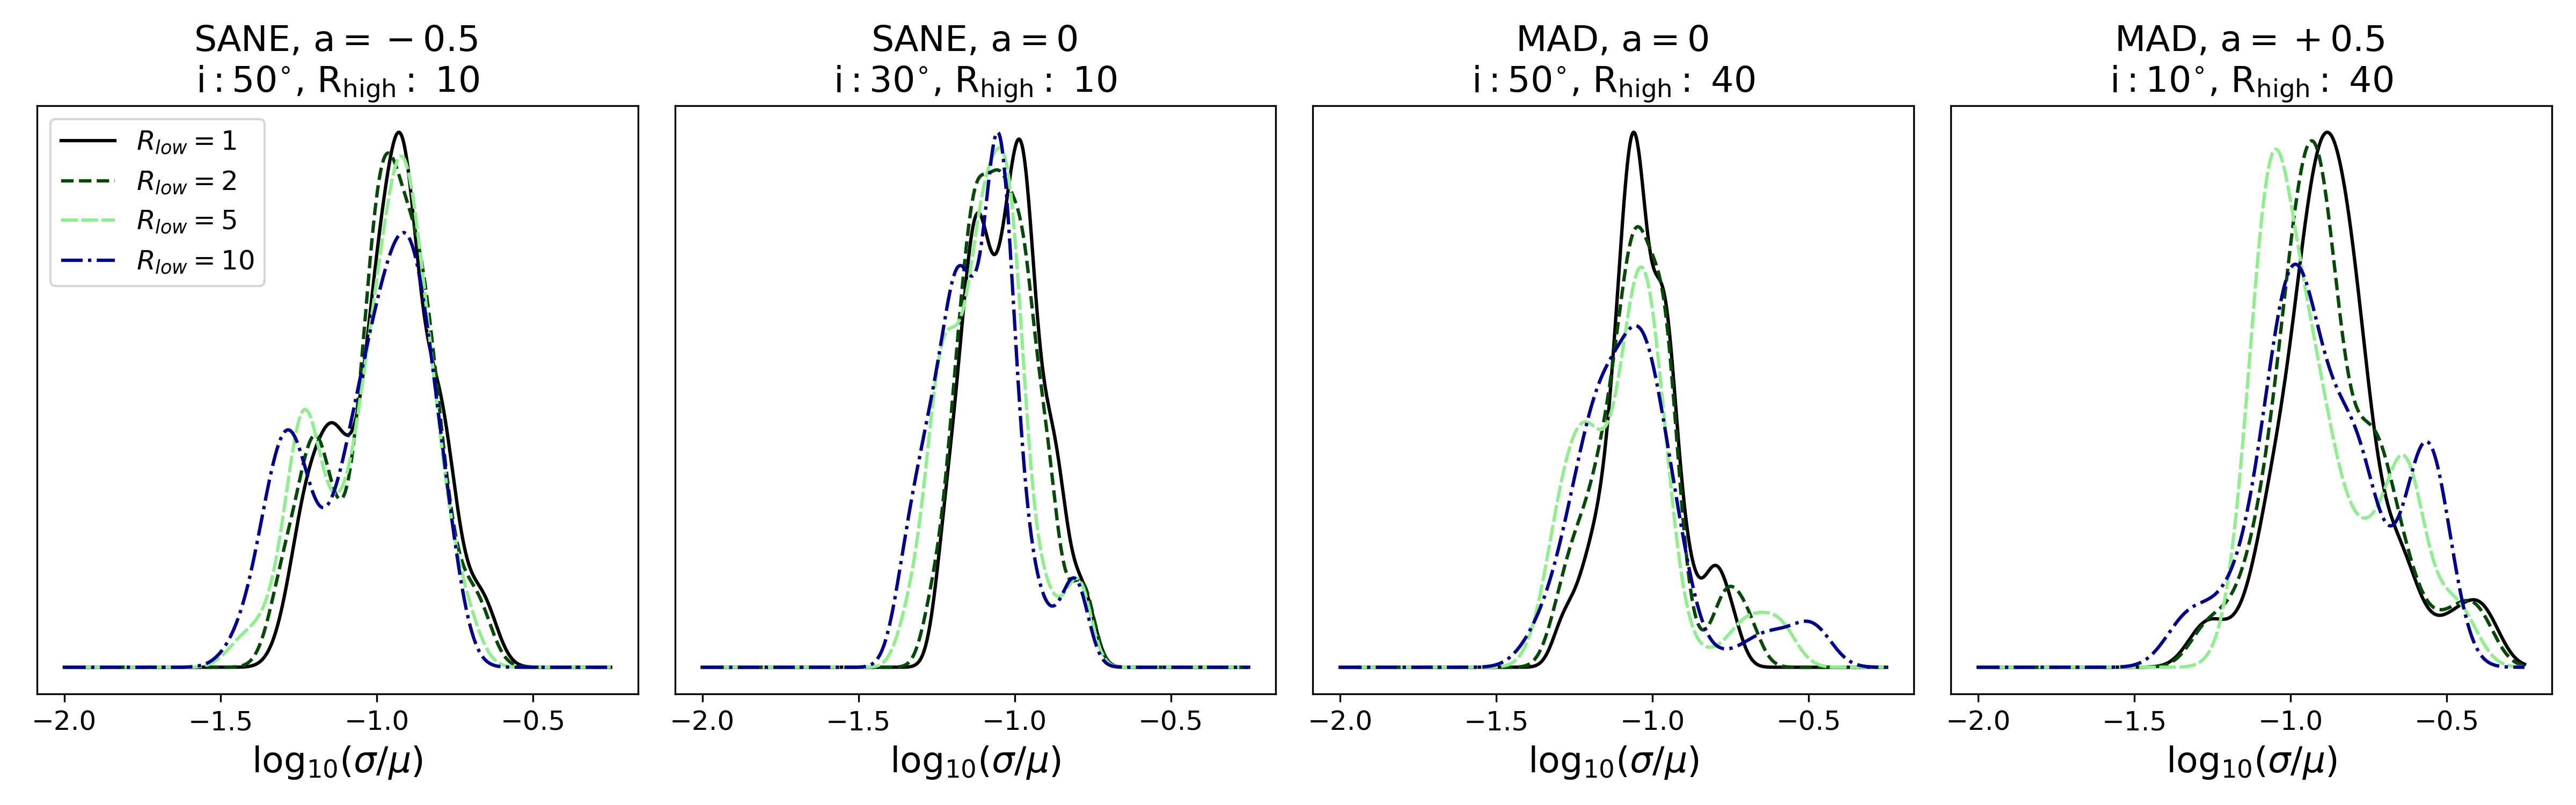
\includegraphics[width=0.95\textwidth]{figures/mi_rlow_select_models.png}
  \caption{Modulation index computed over 3 hour intervals $\mi{3}$ for a subset of the thermal models (\kharma datasets).
For this analysis, we considered the 25,000--30,000$\tg$ time interval.}
  \label{fig:mi_rlow}
\end{figure*}

%==============================================================================
\subsection{Effect of self-consistent electron heating}

\citealt{10.1093/mnras/stv2084} provide a formulation to model electron thermodynamics during the fluid evolution.
Numerical dissipation at the grid scale sources entropy generation and is used to heat the electrons based on a microphysical, sub-grid heating prescription.
Local fluid and electromagnetic variables are used to compute the electron entropy which, along with the ideal gas equation of state, can be converted into a temperature $\Theta_{e}$.
This approach allows computing the electron temperature at each timestep of the simulation rather than post-processing, as is done in the $\Rh$ and Critical-$\beta$ prescriptions.

We consider three sub-grid heating models that prescribe the partition of dissipated energy into electrons and ions.
\cite{2010MNRAS.409L.104H} computed the ratio of ion-to-electron heating due to dissipation of Alfv\'enic turbulent cascade, while \cite{10.1093/mnras/stx2530} and \cite{Rowan_2017} considered magnetic reconnection as the source of energy dissipation at sub-grid scales.
These studies provide approximate fitting formulae for the ion-to-electron heating rate $Q_{i}/Q_{e}$ based on local ion-to-electron temperature ratio $T_{i}/T_{e}$ and local magnetic field strength---parameterized by $\sigma$ or $\beta$.

We use a subset of the simulations analyzed in \citealt{2020MNRAS.494.4168D}.
These include MAD and SANE accretion flows at spins, $\abh = 0,+1/2,+15/16$.
We compute the 3 hour modulation index $\mi{3}$, over the time interval 5,000--10,000$GM/c^{3}$.
The average $\mi{3}$ values are comparable to similar $\Rh$ models, with SANE reconnection models exhibiting a slightly reduced variability as compared to the corresponding turbulent heating models.
However, the $\mi{3}$ distribution is still inconsistent with the historical data.

%==============================================================================
\subsection{Effect of fluid adiabatic index}

We expect the ions and electrons in hot accretion flows to be thermally decoupled and the resulting plasma to be two-temperature \citep{1976ApJ...204..187S, Quataert_1998, 10.1093/mnras/stw3116, Ryan_2018, Chael2018}.
The electrons are relativistic and can be modeled as a fluid with an adiabatic index $\Gamma_{e}=4/3$, while the ions are nonrelativistic with adiabatic index $\Gamma_{i}=5/3$.

The adiabatic index of the fluid assumes a value between $\Gamma_{e}$ and $\Gamma_{i}$ dictated by the thermodynamics of the ions and electrons (cf. Figure 4 in \citealt{10.1093/mnras/stw3116}).
If the electrons and ions have equal temperature then in the relativistic electron/nonrelativistic ion regime the fluid adiabatic index is 13/9.

Our simulations are not fully consistent in their treatment of the adiabatic index.
All use a fixed $\Gamma_\mathrm{ad}$, but some set $\Gamma_\mathrm{ad} = 4/3$ while other use $13/9$ or $5/3$.

Two-temperature simulations can self-consistently evolve adiabatic indices of electrons and ions and compute the net fluid adiabatic index with contributions from both species \citep{10.1093/mnras/stw3116}.
These two-temperature simulations often show variation of the adiabatic index with polar angle, with the fluid energy dominated by hot electrons near the poles ($\Gamma = 4/3$) and by cooler ions and  electrons in the midplane ($\Gamma=5/3$).

We evaluate the effect of $\Gamma_\mathrm{ad}$ on light curve variability by comparing $\mi{3}$ for thermal, GRMHD simulations with varying  $\Gamma_\mathrm{ad}$.
This includes MAD models with $\Gamma_\mathrm{ad}=13/9$ (see Section~\ref{app:narayan} and  \citealt{2021arXiv210812380N}) and SANE models with $\Gamma_\mathrm{ad}=5/3$.
The models exhibit light curve variability similar to the fiducial models and all have \mi{3} distributions that are inconsistent with the historical data.

\subsection{Effect of resolution}

For the 50\% change in resolution considered in the comparison shown in the preceding Appendix (between \kharma and \bhac simulations) we find no
evidence for systematic changes in \mi{3} with resolution.  This is not a large
range in resolution, however, and much higher resolution simulations \citep{2022ApJ...924L..32R, 2020ApJ...900..100R, 2021arXiv211103689N} 
show the emergence of qualitatively
new structures (plasmoids) in current sheets that could affect 230GHz variability.
A deeper study of the resolution dependence of variability is clearly warranted
but is beyond the scope of this paper.
